\chapter{Specifikacija programske potpore}
		
	\section{Funkcionalni zahtjevi}
			
			\textbf{\textit{dio 1. revizije}}\\
			
			\textit{Navesti \textbf{dionike} koji imaju \textbf{interes u ovom sustavu} ili  \textbf{su nositelji odgovornosti}. To su prije svega korisnici, ali i administratori sustava, naručitelji, razvojni tim.}\\
				
			\textit{Navesti \textbf{aktore} koji izravno \textbf{koriste} ili \textbf{komuniciraju sa sustavom}. Oni mogu imati inicijatorsku ulogu, tj. započinju određene procese u sustavu ili samo sudioničku ulogu, tj. obavljaju određeni posao. Za svakog aktora navesti funkcionalne zahtjeve koji se na njega odnose.}\\
			
			
			\noindent \textbf{Dionici:}
			
			\begin{packed_enum}
				
				\item Dionik 1
				\item Dionik 2				
				\item ...
				
			\end{packed_enum}
			
			\noindent \textbf{Aktori i njihovi funkcionalni zahtjevi:}
			
			
			\begin{packed_enum}
				\item  \underbar{Aktor 1 (inicijator) može:}
				
				\begin{packed_enum}
					
					\item funkcionalnost 1
					\item funkcionalnost 2
					\begin{packed_enum}
						
						\item  podfunkcionalnost 1 
						\item  podfunkcionalnost 2
				
					\end{packed_enum}
					\item  funkcionalnost 3
					
				\end{packed_enum}
			
				\item  \underbar{Aktor 2 (sudionik) može:}
				
				\begin{packed_enum}
					
					\item funkcionalnost 1
					\item funkcionalnost 2
					
				\end{packed_enum}
			\end{packed_enum}
			
			\eject 
			
			
				
			\subsection{Obrasci uporabe}
				
				\textbf{\textit{dio 1. revizije}}
				
				\subsubsection{Opis obrazaca uporabe}
					\textit{Funkcionalne zahtjeve razraditi u obliku obrazaca uporabe. Svaki obrazac je potrebno razraditi prema donjem predlošku. Ukoliko u nekom koraku može doći do odstupanja, potrebno je to odstupanje opisati i po mogućnosti ponuditi rješenje kojim bi se tijek obrasca vratio na osnovni tijek.}\\
					

					\noindent \underbar{\textbf{UC$<$broj obrasca$>$ -$<$ime obrasca$>$}}
					\begin{packed_item}
	
						\item \textbf{Glavni sudionik: }$<$sudionik$>$
						\item  \textbf{Cilj:} $<$cilj$>$
						\item  \textbf{Sudionici:} $<$sudionici$>$
						\item  \textbf{Preduvjet:} $<$preduvjet$>$
						\item  \textbf{Opis osnovnog tijeka:}
						
						\item[] \begin{packed_enum}
	
							\item $<$opis korak jedan$>$
							\item $<$opis korak dva$>$
							\item $<$opis korak tri$>$
							\item $<$opis korak četiri$>$
							\item $<$opis korak pet$>$
						\end{packed_enum}
						
						\item  \textbf{Opis mogućih odstupanja:}
						
						\item[] \begin{packed_item}
	
							\item[2.a] $<$opis mogućeg scenarija odstupanja u koraku 2$>$
							\item[] \begin{packed_enum}
								
								\item $<$opis rješenja mogućeg scenarija korak 1$>$
								\item $<$opis rješenja mogućeg scenarija korak 2$>$
								
							\end{packed_enum}
							\item[2.b] $<$opis mogućeg scenarija odstupanja u koraku 2$>$
							\item[3.a] $<$opis mogućeg scenarija odstupanja  u koraku 3$>$
							
						\end{packed_item}
					\end{packed_item}
					
					\noindent \underbar{\textbf{UC -}}
					\begin{packed_item}
						
						\item \textbf{Glavni sudionik: }
						\item  \textbf{Cilj:} 
						\item  \textbf{Sudionici:} 
						\item  \textbf{Preduvjet:} 
						\item  \textbf{Opis osnovnog tijeka:}
						
						\item[] \begin{packed_enum}
							
							\item 
							\item 
							\item 
							\item 
							\item 
						\end{packed_enum}
						
						\item  \textbf{Opis mogućih odstupanja:}
						
						\item[] \begin{packed_item}
							
							\item[2.a] 
							\item[] \begin{packed_enum}
								
								\item 
								\item
								
							\end{packed_enum}
							\item[2.b] 
							\item[3.a] 
							
						\end{packed_item}
					\end{packed_item}
				
					\noindent \underbar{\textbf{UC1 - Pregled recepata}}
					\begin{packed_item}
						
						\item \textbf{Glavni sudionik: Neregistiran korisnik, Registriran korisnik}
						\item  \textbf{Cilj: Pregled recepata temeljem kategorija} 
						\item  \textbf{Sudionici: Baza podataka} 
						\item  \textbf{Preduvjet: -} 
						\item  \textbf{Opis osnovnog tijeka:}
						
						\item[] \begin{packed_enum}
							
							\item Korisnik otvori platformu
							\item Ponuđene su mu kategorije, vrste kuhinje, specifični sastojci
							\item Korisnik odabire kategoriju i prikazuju mu se recepti
						\end{packed_enum}
						
						\item  \textbf{Opis mogućih odstupanja:}
						
						\item[] \begin{packed_item}
							
							\item[2.a] 
							\item[] \begin{packed_enum}
								
								\item 
								\item
								
							\end{packed_enum}
							\item[2.b] 
							\item[3.a] 
							
						\end{packed_item}
					\end{packed_item}
					
					
					\noindent \underbar{\textbf{UC2 - Registracija}}
					\begin{packed_item}
						
						\item \textbf{Glavni sudionik: Neregistrirani korisnik}
						\item  \textbf{Cilj: Stvaranje računa za pristup ostalim značajkama sustava}  
						\item  \textbf{Sudionici: Baza podtaka} 
						\item  \textbf{Preduvjet:-} 
						\item  \textbf{Opis osnovnog tijeka:}
						
						\item[] \begin{packed_enum}
							
							\item Korisnik odabire opciju za registraciju
							\item Korisnik unosi potrebne korisničke podatke
							\item Korisnik prima obavijest o uspješnoj registraciji
						\end{packed_enum}
						
						\item  \textbf{Opis mogućih odstupanja:}
						
						\item[] \begin{packed_item}
							
							\item[2.a] Odabir već zauzetog korisničkog imena i/ili e-maila, unos korisničkog podatka u nedozvoljenom formatu ili pružanje neispravnoga e-maila
							\item[] \begin{packed_enum}
								
								\item  Sustav obavještava korisnika o neuspjelom upisu i vraća ga na stranicu za registraciju
								\item Korisnik mijenja potrebne podatke te završava unos ili odustaje od registracije
								
							\end{packed_enum}
							
						\end{packed_item}
					\end{packed_item}
					
					
					\noindent \underbar{\textbf{UC3 - Prijava u sustav}}
					\begin{packed_item}
						
						\item \textbf{Glavni sudionik: }
						\item  \textbf{Cilj:} 
						\item  \textbf{Sudionici:} 
						\item  \textbf{Preduvjet:} 
						\item  \textbf{Opis osnovnog tijeka:}
						
						\item[] \begin{packed_enum}
							
							\item 
							\item 
							\item 
							\item 
							\item 
						\end{packed_enum}
						
						\item  \textbf{Opis mogućih odstupanja:}
						
						\item[] \begin{packed_item}
							
							\item[2.a] 
							\item[] \begin{packed_enum}
								
								\item 
								\item
								
							\end{packed_enum}
							\item[2.b] 
							\item[3.a] 
							
						\end{packed_item}
					\end{packed_item}
					
					\noindent \underbar{\textbf{UC4 - Objava recepata}}
					\begin{packed_item}
						
						\item \textbf{Glavni sudionik: Registrirani korisnik }
						\item  \textbf{Cilj: Objava svog recepta na stranici} 
						\item  \textbf{Sudionici:} 
						\item  \textbf{Preduvjet: Registracija i prijava korisnika} 
						\item  \textbf{Opis osnovnog tijeka:}
						
						\item[] \begin{packed_enum}
							
							\item 
							\item 
							\item 
							\item 
							\item 
						\end{packed_enum}
						
						\item  \textbf{Opis mogućih odstupanja:}
						
						\item[] \begin{packed_item}
							
							\item[2.a] 
							\item[] \begin{packed_enum}
								
								\item 
								\item
								
							\end{packed_enum}
							\item[2.b] 
							\item[3.a] 
							
						\end{packed_item}
					\end{packed_item}
					
					\noindent \underbar{\textbf{UC5 - Razmjena poruka}}
					\begin{packed_item}
						
						\item \textbf{Glavni sudionik: }
						\item  \textbf{Cilj:} 
						\item  \textbf{Sudionici:} 
						\item  \textbf{Preduvjet:} 
						\item  \textbf{Opis osnovnog tijeka:}
						
						\item[] \begin{packed_enum}
							
							\item 
							\item 
							\item 
							\item 
							\item 
						\end{packed_enum}
						
						\item  \textbf{Opis mogućih odstupanja:}
						
						\item[] \begin{packed_item}
							
							\item[2.a] 
							\item[] \begin{packed_enum}
								
								\item 
								\item
								
							\end{packed_enum}
							\item[2.b] 
							\item[3.a] 
							
						\end{packed_item}
					\end{packed_item}
					
					\noindent \underbar{\textbf{UC6 - Čavrljanje }}
					\begin{packed_item}
						
						\item \textbf{Glavni sudionik: }
						\item  \textbf{Cilj:} 
						\item  \textbf{Sudionici:} 
						\item  \textbf{Preduvjet:} 
						\item  \textbf{Opis osnovnog tijeka:}
						
						\item[] \begin{packed_enum}
							
							\item 
							\item 
							\item 
							\item 
							\item 
						\end{packed_enum}
						
						\item  \textbf{Opis mogućih odstupanja:}
						
						\item[] \begin{packed_item}
							
							\item[2.a] 
							\item[] \begin{packed_enum}
								
								\item 
								\item
								
							\end{packed_enum}
							\item[2.b] 
							\item[3.a] 
							
						\end{packed_item}
					\end{packed_item}
					
					\noindent \underbar{\textbf{UC7 - Videopoziv}}
					\begin{packed_item}
						
						\item \textbf{Glavni sudionik: }
						\item  \textbf{Cilj:} 
						\item  \textbf{Sudionici:} 
						\item  \textbf{Preduvjet:} 
						\item  \textbf{Opis osnovnog tijeka:}
						
						\item[] \begin{packed_enum}
							
							\item 
							\item 
							\item 
							\item 
							\item 
						\end{packed_enum}
						
						\item  \textbf{Opis mogućih odstupanja:}
						
						\item[] \begin{packed_item}
							
							\item[2.a] 
							\item[] \begin{packed_enum}
								
								\item 
								\item
								
							\end{packed_enum}
							\item[2.b] 
							\item[3.a] 
							
						\end{packed_item}
					\end{packed_item}
					
					
				\subsubsection{Dijagrami obrazaca uporabe}
					
					\textit{Prikazati odnos aktora i obrazaca uporabe odgovarajućim UML dijagramom. Nije nužno nacrtati sve na jednom dijagramu. Modelirati po razinama apstrakcije i skupovima srodnih funkcionalnosti.}
				\eject		
				
			\subsection{Sekvencijski dijagrami}
				
				\noindent
				\textbf{Obrazac uporabe UC1-Pregled recepata}\newline
					{Korisnik šalje zahtjev za prikaz recepata po kategorijama, sastojcima i/ili kuhinjama kojim pripadaju. Poslužitelj dohvaća recepete koji zadovoljavaju uvjete i prikazuje ih korisniku. Korisnik sada može spremiti recepte, ako je prijavljen to se provodi, ako nije preusmjeri ga se na stranicu za prijavu.}
				\eject
				
				\begin{figure}[H]
					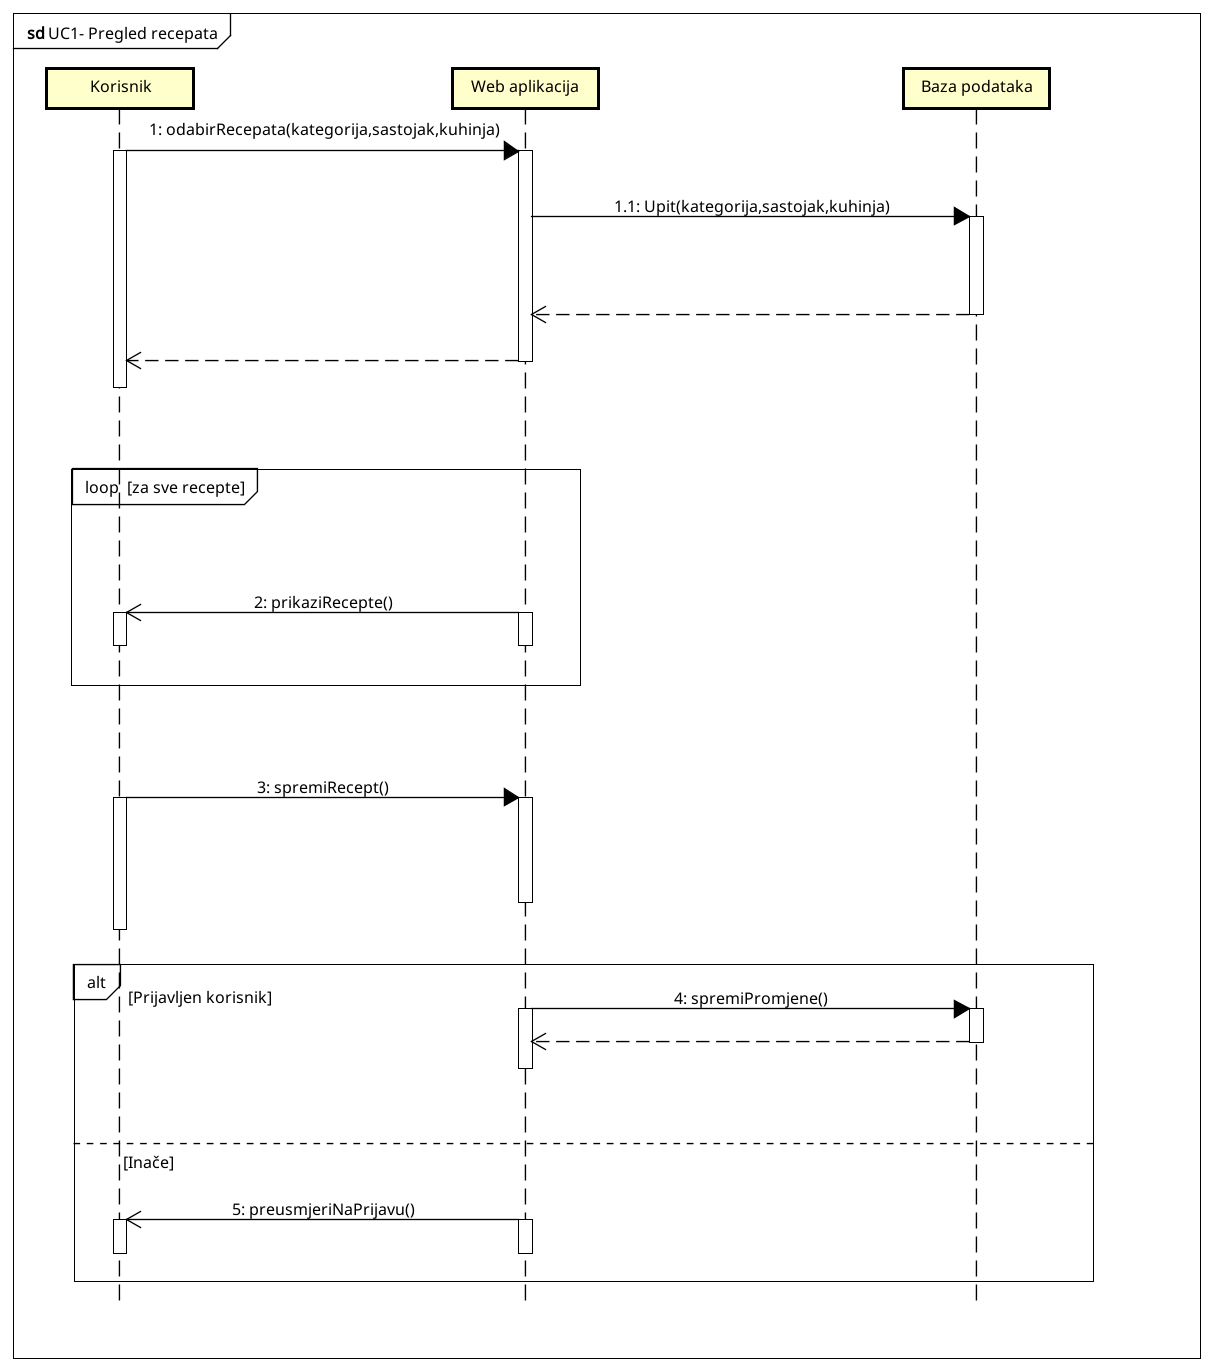
\includegraphics[scale= 0.5]{slike/sekvencijski_dijagramUC1.png}
					\centering
					\caption{Sekvencijski dijagram za UC1}
					\label{fig:Sekvencijski dijagram za UC1}
				\end{figure} 
				\eject

				\noindent
				\textbf{Obrazac uporabe UC3-Registracija}\newline
					{Korisnik se registrira s korisničkim imenom i lozinkom. Ako takav korisnik već postoji, korisniku se ispisuje greška. Inače, korisnik se uspješno registrirao i to se bilježi u bazi podataka.}
				\eject

				\begin{figure}[H]
					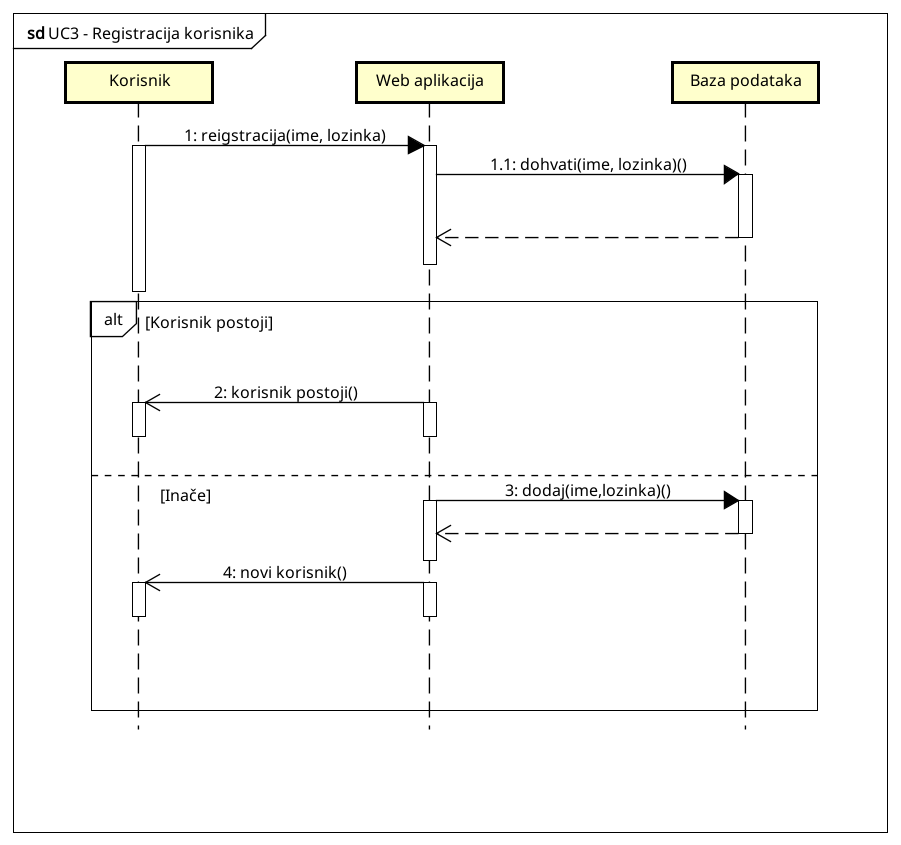
\includegraphics[scale= 0.6]{slike/sekvencijski_dijagramUC3.png}
					\centering
					\caption{Sekvencijski dijagram za UC3}
					\label{fig:Sekvencijski dijagram za UC3}
				\end{figure}
				
				\eject

				\noindent
				\textbf{Obrazac uporabe UC4-Prijava Korisnika}\newline
					{Korisnik pokuša objaviti novi recept. Ako nije prijavljen, preusmjeri ga se na prijavu. Inače, recept se dodaje u bazu podataka i o tome se obavijesti korisnik.}
				\eject

				\begin{figure}[H]
					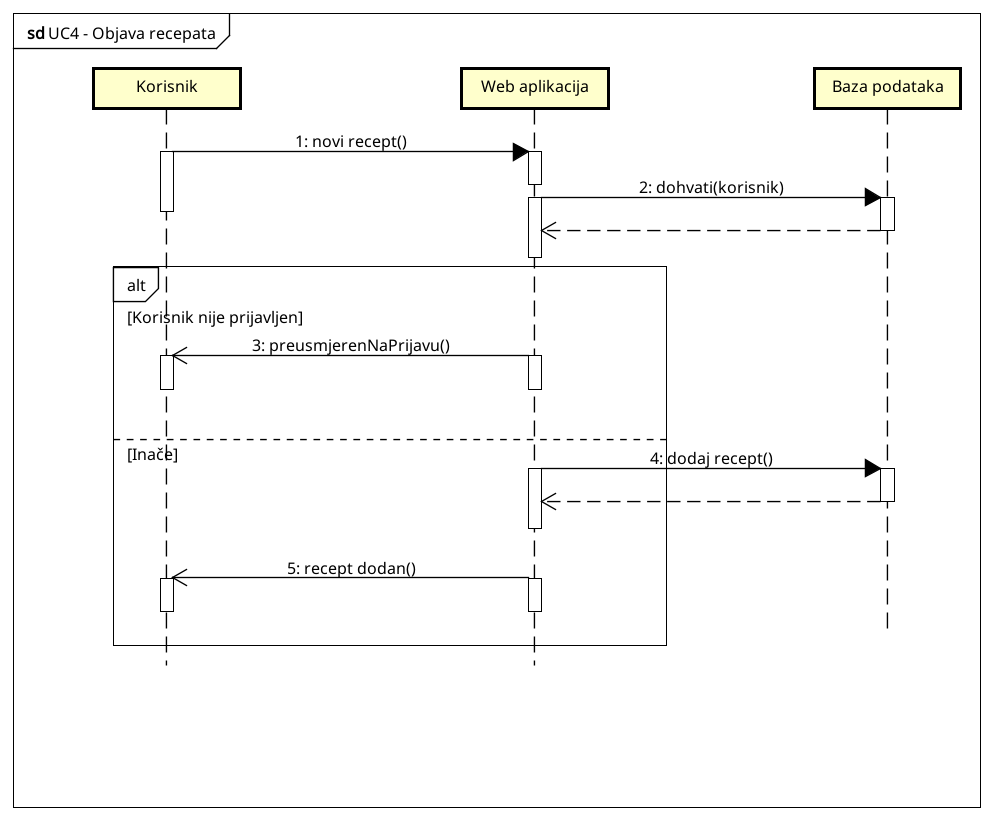
\includegraphics[scale= 0.6]{slike/sekvencijski_dijagramUC4.png}
					\centering
					\caption{Sekvencijski dijagram za UC4}
					\label{fig:Sekvencijski dijagram za UC4}
				\end{figure}

				\eject

				\noindent
				\textbf{Obrazac uporabe UC8-Videopoziv}\newline
					{Korisnik zatraži video poziv s drugim korisnikom. Ako drugi korisnik ne postoji, poziv se ne uspostavlja i o tome se obavijesti prvog korisnika. Inače se šalje zahtjev za video pozivom drugom korisniku, koji ga može odbiti ili prihvatiti. Ako odbije poziv se ne uspostavlja i o tome se obavijesti prvi korsnik. Ako prihvati uspostavi se video poziv između dva korisnika.}
				\eject

				\begin{figure}[H]
					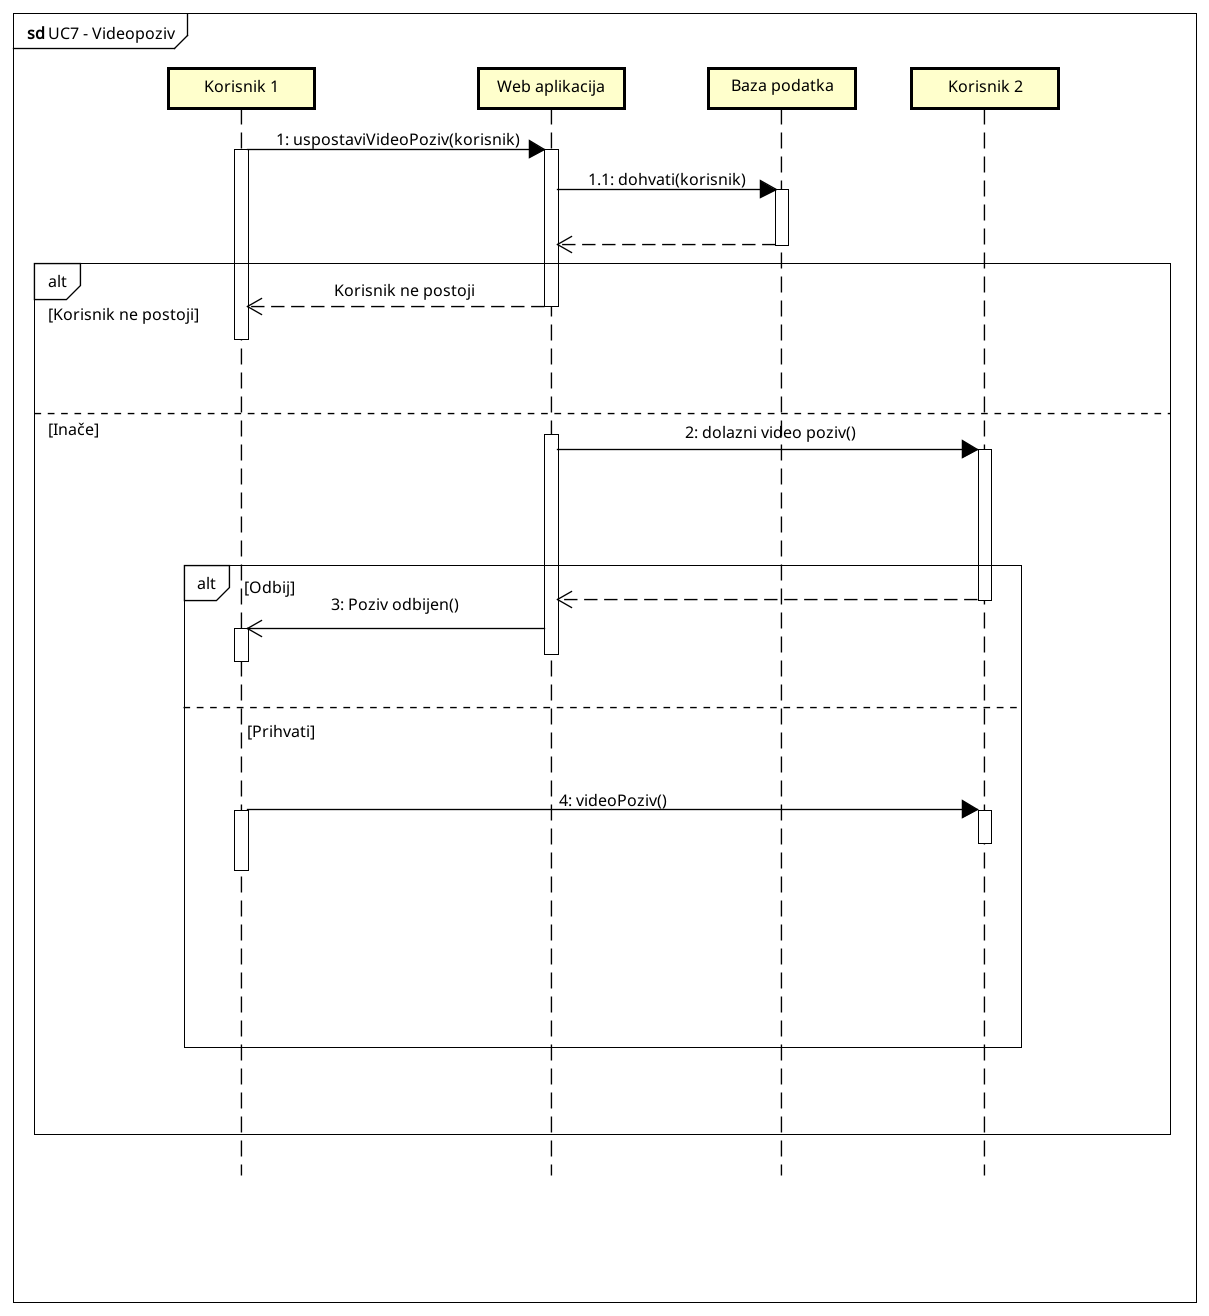
\includegraphics[scale= 0.5]{slike/sekvencijski_dijagramUC7.png}
					\centering
					\caption{Sekvencijski dijagram za UC7}
					\label{fig:Sekvencijski dijagram za UC7}
				\end{figure}
				
				\eject
			
			\section{Ostali zahtjevi}
		
			\textbf{\textit{dio 1. revizije}}\\
		 
			 \textit{Nefunkcionalni zahtjevi i zahtjevi domene primjene dopunjuju funkcionalne zahtjeve. Oni opisuju \textbf{kako se sustav treba ponašati} i koja \textbf{ograničenja} treba poštivati (performanse, korisničko iskustvo, pouzdanost, standardi kvalitete, sigurnost...). Primjeri takvih zahtjeva u Vašem projektu mogu biti: podržani jezici korisničkog sučelja, vrijeme odziva, najveći mogući podržani broj korisnika, podržane web/mobilne platforme, razina zaštite (protokoli komunikacije, kriptiranje...)... Svaki takav zahtjev potrebno je navesti u jednoj ili dvije rečenice.}
			 
			 
			 
	